%flowchart%%%%%%%%%%%%%%%%%%%%%%%%%%%%%%%%%%%%%%%%%%%%%%%%%%%%%%%%%%%%%%%%%%%%%%%%%%%%%%%%
%2345678901234567890123456789012345678901234567890123456789012345678901234567890
%        1         2         3         4         5         6         7         8

\documentclass[letterpaper, 10 pt, conference]{ieeeconf}  % Comment this line out if you need a4paper

%\documentclass[a4paper, 10pt, conference]{ieeeconf}      % Use this line for a4 paper

\IEEEoverridecommandlockouts                              % This command is only needed if 
                                                          % you want to use the \thanks command

\overrideIEEEmargins                                      % Needed to meet printer requirements.

% See the \addtolength command later in the file to balance the column lengths
% on the last page of the document

% The following packages can be found on http:\\www.ctan.org
%\usepackage{graphics} % for pdf, bitmapped graphics files
%\usepackage{epsfig} % for postscript graphics files
%\usepackage{mathptmx} % assumes new font selection scheme installed
%\usepackage{times} % assumes new font selection scheme installed
\usepackage{amsmath} % assumes amsmath package installed
%\usepackage{amssymb}  % assumes amsmath package installed
\usepackage{graphicx}
\usepackage{times,ifthen}
\usepackage{algorithm}
\usepackage{algorithmic}
%\usepackage{algorithmicx}
\usepackage{multirow}
\usepackage{tabularx}

\title{\LARGE \bf
 Distributed network localization
}


\author{Laurent Fasnacht, Matteo Pagliardini, Bernard Maccari% <-this % stops a space
%\thanks{*This work was not supported by any organization}% <-this % stops a space
%\thanks{$^{1}$Albert Author is with Faculty of Electrical Engineering, Mathematics and Computer Science,
%        University of Twente, 7500 AE Enschede, The Netherlands
%        {\tt\small albert.author@papercept.net}}%
%\thanks{$^{2}$Bernard D. Researcheris with the Department of Electrical Engineering, Wright State University,
 %       Dayton, OH 45435, USA
%        {\tt\small b.d.researcher@ieee.org}}%
}


\begin{document}



\maketitle
\thispagestyle{empty}
\pagestyle{empty}


%%%%%%%%%%%%%%%%%%%%%%%%%%%%%%%%%%%%%%%%%%%%%%%%%%%%%%%%%%%%%%%%%%%%%%%%%%%%%%%%
\begin{abstract}
This paper presents an implementation of a fully distributed algorithm for localizing static sensor nodes relative to each other in a random two-dimensional network. Nodes can sense noisy distances to neighboring nodes and communicate asynchronously with them. \\
Our method follow the work of David Moore \emph{et al.} \cite{MooreTeller}, which uses robust quadrilaterals and trilateration to localize nodes, relative to fixed anchors. We extend this method to allow nodes to select a good set of anchors, and to handle different variances for each measurement. \\
Using simulation, we evaluate our method in term of speed of convergence and precision of the estimated positions. We show that this method is robust even in a very noisy environment, and that it's able to relocalize moved nodes quickly.\\
\end{abstract}


%%%%%%%%%%%%%%%%%%%%%%%%%%%%%%%%%%%%%%%%%%%%%%%%%%%%%%%%%%%%%%%%%%%%%%%%%%%%%%%%
\section{Introduction}

Self-localization is a fundamental need in networks, which has numerous applications such as environmental monitoring or surveillance. Absolute localization (GPS for instance) is often unavailable, because of cost or energy constraints. However, relative localization, which is done using local distance measurements between nodes may be enough. It has to be made in a distributed way in order to minimize communications and computation, which are energy-consuming. Relative localization in a distributed way is non-trivial, since each node has only a very limited knowledge of the system, but also provides robustness, since no node is a single point of failure.

In this report, we will try to locate nodes in a 2D network, in which nodes can measure a noisy distance to their neighbors.

The basic idea would be to use trilateration to localize a node. However, this method is very sensitive to noise, as noise produces flex and flip ambiguities (see figure 3 in \cite{MooreTeller}). Our solution is based on the idea of David Moore \emph{et al.} \cite{MooreTeller}, which restricts trilateration to happen in \emph{robust quadrilaterals}. A \emph{robust quadrilateral} is a quadrilateral $ABCD$ in which any node can communicate to any other, and any triangle formed by three of these points is such that $b \cdot \sin(\min_i \theta_i)^2 > d_{min} $ where the $\theta_i$ are the angles of the triangle, $b$ the smallest side length, and $d_{min}$ a constant depending on the measurement noise. By constructing chains of robust quadrilaterals (each robust quadrialateral which contain three nodes in common with the previous one), we can localize reliabily each node in the chain. The algorithm in the original paper doesn't require anchors, but doesn't provide a way of computing network-wide coordinates.

In this paper, we present a MATLAB implementation of a slightly extended version of this algorithm, which has the following caracteristics:

\begin{enumerate}
    \item It's designed to handle noisy distance measurements, with unknown variance.
    \item It is fully distributed, requiring no beacons or anchors, and provides network-wide coordinates for every localized node in the network
    \item It localizes each node correctly with high probability, or not at all.
\end{enumerate}

We will then evaluate this algorithm, using various networks with different caracteristics. We will use the following performance metrics:

\begin{itemize}
    \item The number of nodes localized.
    \item The mean-square error in Euclidean 2D space for the location of nodes
    \item The mean-square error for the distances between nodes
\end{itemize}

We took care to be sure that our implementation is fully distributed, which means that it would be easily feasible to implement the algorithm in real sensor nodes.



%We present a solution to localize a network of static sensor nodes. The nodes can sense noisy distances to neighboring nodes and are also capable of communicating with their neighbors. We consider the quality of the algorithm looking at several criteria such as precision, speed of convergence, stability, resistance to perturbations, scalability and computational cost. A good localization algorithm has to balance all of these aspects.


%Our method demonstrated the following capabilities : INSERT RESULTS HERE | INSERT RESULTS HERE | INSERT RESULTS HERE | INSERT RESULTS HERE | INSERT RESULTS HERE | INSERT RESULTS HERE | INSERT RESULTS HERE | INSERT RESULTS HERE | INSERT RESULTS HERE | INSERT RESULTS  

\subsection{Modifications over Moore \emph{et al's} implementation}

Since we didn't implemented exactly what was described in the paper, we will present here what was made differently.

%%%%%%%%%%%%%%%%%%%%%%%%%%%% ROBUST QUADS %%%%%%%%%%%%%%%%%%%%%%%%%%%%%%%%%%%%%%%%%%%%%%%%
\subsubsection{Robust quadrilateral detection}

One of the main part of the algorithm is to detect all robust quadrilaterals for a given node. Algorithm 1 in \cite{MooreTeller} has a complexity of $O(m^4)$, where $m$ is the number of edges. 

Saving computational time is an important aspect of sensors networks, as it means sparing energy.

Since all three are by definition neighbors of the first node, we can implement it in $O(m^3)$ (which gives exactly the same results as the original algorithm), see algorithm \ref{algo1}.

\begin{algorithm}
\caption{\label{algo1}Find robust quads of node $i$. This algorithm loops over each triplet of neighbours of the node $i$ and find if the resulting quad is robust. $quadIsRobust$ checks if the quad is fully connected, and if each triangle of the quad is robust.}
\begin{algorithmic} 
\STATE $neighboursIds \leftarrow neighbors(node(i))$
\STATE $nbneighbours \leftarrow length(neighboursIds)$ 
\STATE $robustQuadsList \leftarrow []$ 
\FOR  {$j_i=0$ to $ nbneighbours $} 
\FOR  {$k_i=j_i+1$ to $ nbneighbours $} 
\FOR  {$l_i=k_i+1$ to $ nbneighbours $} 
\STATE $j \leftarrow neighboursIds(j_i)$ 
\STATE $k \leftarrow neighboursIds(k_i)$
\STATE $l \leftarrow neighboursIds(l_i)$ \newline
\IF {$quadIsRobust(i,j,k,l)$} 
\STATE $robustQuadsList \leftarrow [i, j, k, l]$
\ENDIF 
\newline
\ENDFOR
\ENDFOR
\ENDFOR 
\STATE $node(i).robustquads \leftarrow robustQuadsList$
\end{algorithmic}
\end{algorithm}

%%%%%%%%%%%%%%%%%%%%%%%%%%%% VAR ESTIMATION %%%%%%%%%%%%%%%%%%%%%%%%%%%%%%%%%%%%%%%%%%%%%%%
\subsubsection{Robust quadrilateral criteria}

In \cite{MooreTeller}, the authors use as a  $b \cdot \sin(\min_i \theta_i)^2 > d_{min}$, an propose that $d_{min}=3\sigma$. This works as long as the noise is the same for all edges. 

In our case, we based our hypothesis that $\sigma$ is proportional to the length of the measurement.

We used therefore $\sin(\min_i \theta_i)^2 > d_{mf} \sigma$, where $d_{mf}$ is a constant.

\subsubsection{Variance estimation}

In a real implementation, noise levels are not known a priori. Therefore we implemented, for each edge of the graph, the online estimator for the mean and variance proposed in \cite{Knuth}. This emphasis the fully distributed approach we've choosen.

\subsubsection{Spring relaxation}

As proposed in \cite{MooreTeller}, we have inplemented the spring relaxation technique to see how it can improve performances. The idea is to put virtual springs between nodes, which lengths are exactly the measured length of the edge. Spring relaxation computes the forces applied to each nodes by the strings linking it to its neighbours. Each force is proportional to the difference between the distances measured and the distances computed with the positions of the nodes. Actually, it correspond to minimizing the potential energy for all the springs, using a gradient descent technique.

The node uses a convex combination between the position obtained by the trilateration, and the position obtained by the spring relaxation. The performances of this optimization is discussed in the result section.

\subsubsection{Anchor node estimation, and position propagation}

In \cite{MooreTeller} the positions are computed cluster-wise, and propagated by solving the best rotation and translation to merge these clusters. This implies a lot of information sharing among the nodes and represents to us a flaw in the distributed scheme we wanted.

Our first attempt to solve this problem was to select 3 arbitrary nodes as anchors, and then locate relatively to them. The problem with this approach is that those node might not be in a robust quadrilateral, and it happens quite often that we don't localize anything (about 40\% of the time, in a complete 20-node graph).

Therefore, we've decided to implement a voting scheme. Each node selects it's ``best'' anchor possible (3 points), and broadcast its choice to its neighbors. When a anchor proposal is received, there are three possibilities:
\begin{itemize}
    \item the anchor is better than the one we have currently: choose this anchor
    \item the anchor is worse than the one we have currently: do nothing
    \item it's the same anchor as the one we have currently, but with a different score: update the score in our local memory.
\end{itemize}

To select the best node, we have to use a metric. We define coordinate system based on the anchor $n_1, n_2, n_3$, such that it makes $n_1$ be the origin, $n_2$ a node on the $x$ axis, and $n_3$ be in the $y>0$ region (it's always possible to build such a coordinate system, as long as the three points are not colinear). The score of the anchor is defined as the sum of:
\begin{itemize}
    \item $\sin(\min_i \theta_i)^2$, in the triangle $n_1, n_2, n_3$
    \item Number of robust quadrilaterals containing $n_2$ and $n_3$ in the neighborhood of $n_1$, divided by the number of robust quadrilaterals containing $n_1$
    \item The number of robust quadrilaterals containing $n_1$
\end{itemize}

This make the collective decision prefers $n_1$ having a large number of robust quadrilaterals, and $n_2$ and $n_3$ such that they form the most equilateral triangle, belonging to the biggest number of robust quads possible. This ensure a good likelihood to have good localization properties.

To localize a node, we use the set of robust quadrilaterals the point belongs to, in which the three other points have known coordinates. When several robust-quads are available we select the best one. Here the notion of best is defined as the one which average edge distance to the anchor is the smallest. Indeed, the robust quadrilaterals closer to the anchor are more reliable than the one far away (because measurement errors accumulate). This is also essential for the convergence of the algorithm, as it ensures that the propagation starts from the anchor, and avoid looping (base a node $n$ localization on nodes which were localized used $n$).

As a consequence of this, we only have one relative coordinate system for all of our nodes instead of one coordinate system for each node as in Moore \emph{et al.'s} implementation. 

\subsection{Implementation choices}

To validate that our implementation is indeed an entirely distributed one, each node has only access to:
\begin{itemize}
    \item its private data
    \item a function to broadcast a message
    \item a function which is called when receiving a message
\end{itemize}

This ensures that a node doesn't accidentally has access to internal state of other nodes, to the simulation variables, or to some global variable. 

Our implementation requires only the node to store information from its neighbors, so its pretty cheap in term of memory requirement.

Our simulator has two states, the first is the computation stage, in which node try to localize, do the measurements, put message in the sending queue. During the second stage the message are processed and notified to the receiving nodes. These two alternated steps ensure a realistic simulation where the information is processed at each timer tick and ensure that we don't do hidden callbacks between nodes. 

Each node can send the the following messages:

\begin{itemize}
    \item measured distances to its neighbours
    \item its absolute position
    %\item its list of robust quads. % Well we don't need it, so don't mention it
    \item the anchor, its score, and the path length (in number of edges) to the anchors
\end{itemize}

\section{Experiments}

We tried to set up simple regular networks, which were used to trivially verify our implementation, removing the uncertainty infered by the graph topology. These graph can as well be used as reference graphs used to compare with more complicated graphs.\newline

%[net]=f_regular_net(20,5,20,gca)
%print -deps '../report/reg1.eps'
%[net]=f_regular_net3(21,5,20,true,gca)
%print -deps '../report/reg3.eps'

\begin{figure}[ht!]
\centering
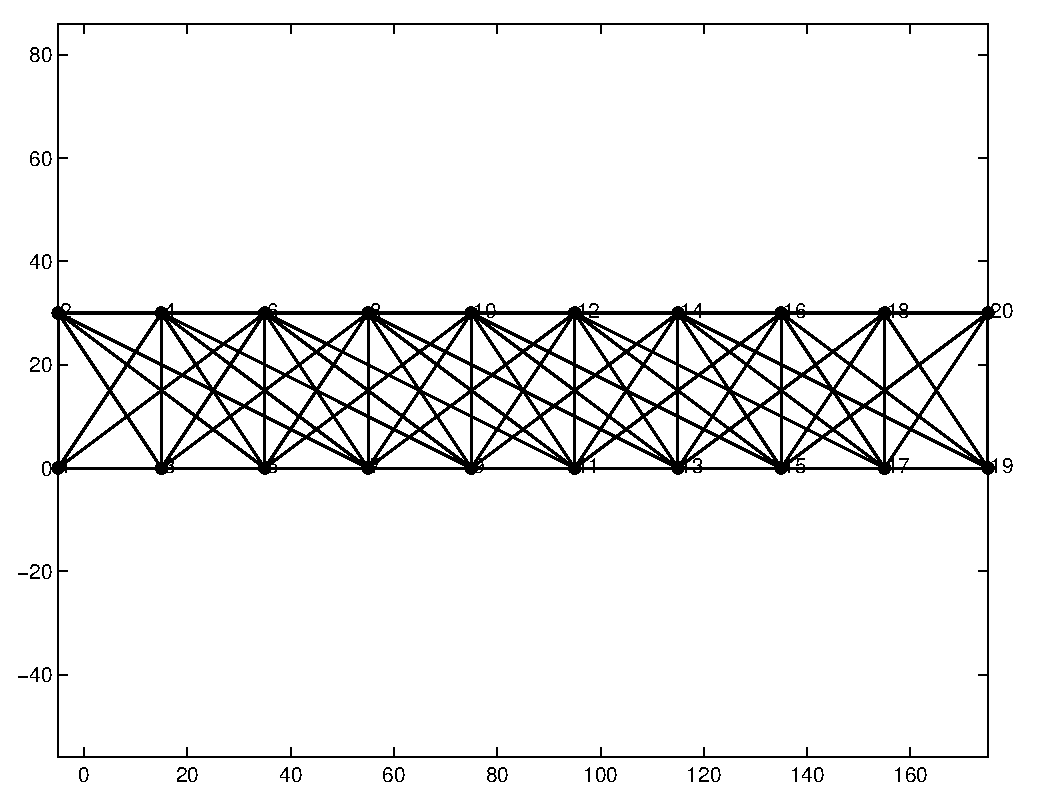
\includegraphics[width=0.4\columnwidth]{reg1.eps} 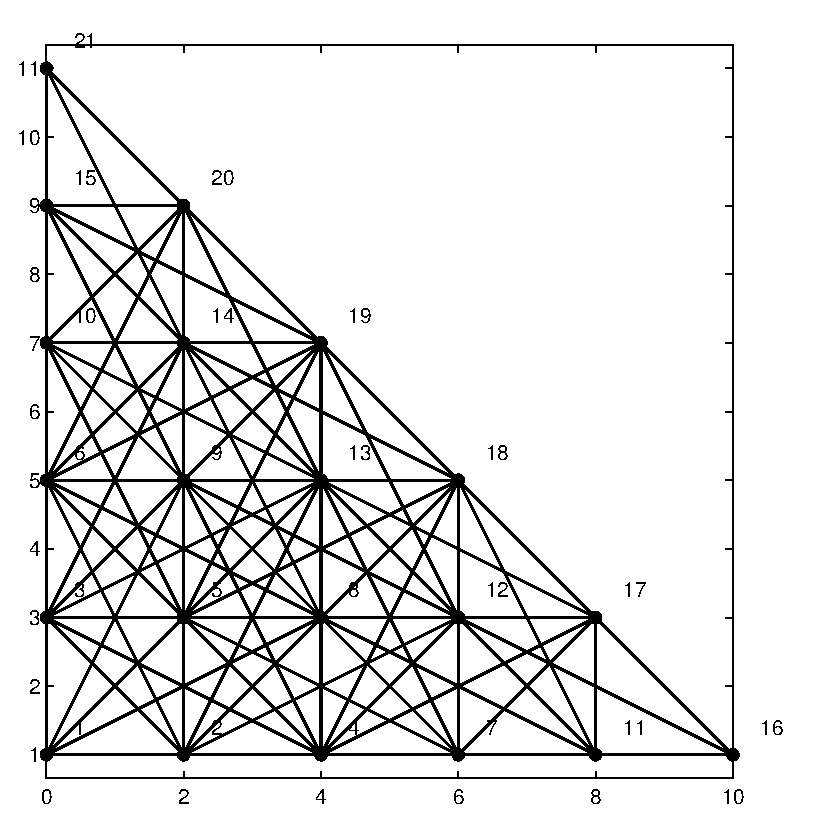
\includegraphics[width=0.4\columnwidth]{reg3.eps}
\caption{Examples of regular graphs}
\end{figure}

\subsection{Parameters}

While regular graphs are useful during developement, it doesn't provide a mean to have statistical data about the efficiency of the algorithm and implementation.

Therefore, we used random graphes, which are generated depending on some parameters. Additionnally, we have parameters specifying the node behaviour, as well as some simulation parameters. All these parameters are listed in table \ref{table:parameters}.

\begin{table}[!hbt]
%Better way to do this?
\begin{tabularx}{8.4cm}{|p{1cm}|p{6.5cm}|}
\hline
\multicolumn{2}{|c|}{Network parameters:} \\
\hline
$N$ & number of nodes \\
$K$ & minimum connectivity \\
$R$ & average communication radius \\
\hline
\multicolumn{2}{|c|}{Node parameters:} \\
\hline
$F$ & probability to do a measurement and broadcast it \\
$d_{mf}$ & ratio between the threshold $d_{min}$ and the variance of the noise \\
$srf$ & spring relaxation factor: weight for the convex combination between the position obtained by trilateration, and the one obtained by spring relaxation. ($srf=0$: no spring relaxation) \\
\hline
\multicolumn{2}{|c|}{Simulation parameters:} \\
\hline
$t_{max}$ & Maximum number of simulation steps \\
$n$ & noise percentage, Gaussian noise on range measurements \\
\hline
\end{tabularx}
\caption{\label{table:parameters}List of parameters}
\end{table}

We used by default the following parameters for all our experiments: 

$N = 20$, $R = 20$, $F = 0.2$, $t_{max} = 100$, $n = 0.1$, $K = 11$, $d_{mf}=1$, $srf \in \{0.0, 0.1\}$

We then tested our implementation with the following set of parameters:

\begin{enumerate}
\item $K \in \{3, 5, 7, 9, 11, 13, 15, 17, 19\}$ (varying connectivity of the graph)
\item $F \in \{0.1, 0.2, 0.3, 0.4, 0.5\}$ (varying communication probability)
\item $n \in \{0.1, 0.2, 0.3, 0.4, 0.5\}$ (varying noise level)
\item $t_{max} = \{1, 2, \ldots 100\}$ (varying the number of iterations)
\end{enumerate}

\section{Results}
%speed of convergence
%Performance Metrics
%Scalability : performances w.r.t Nb of nodes

\section{Conclusion}


\begin{thebibliography}{99}

\bibitem{MooreTeller} David Moore, John Leonard, Daniela Rus, Seth Teller, Robust Distributed Network Localization with Noisy Range Measurements, 2004.

\bibitem{Knuth} Donald Knuth, The Art Of Computer Programming, vol 2, 3rd ed, p. 232





\end{thebibliography}









%%%%%%%%%%%%%%%%%%%%%%%%%%%%%%%%%%%%%%%%%%%%%%%%%%%%%%%%%%%%%%%%%%%%%%
%%%%%%%%%%%%%%% UNDER THIS LINE : OLD STUFF %%%%%%%%%%%%%%%%%%%%%%%%%%
%%%%%%%%%%%%%%%%%%%%%%%%%%%%%%%%%%%%%%%%%%%%%%%%%%%%%%%%%%%%%%%%%%%%%%
OLD STUFF
OLD STUFF
OLD STUFF
OLD STUFF
OLD STUFF














\subsection{Error measurement}
We measure the error on the distances 
%sigma_p
%sigma_d



%spring relaxation :smooth error + decrease convergence speed if bad initalization

\subsection{Perturbations}

\subsection{Shortcomings}
%

\section{Conclusion}











In our implementation the graph can be completely random, however experiments showed that a connectivity threshold of XXX was required to ensure good performances. As in \cite{MooreTeller} we use properties of quadrilaterals to answer the flip ambiguity problem. The flex ambiguity is solved selecting only robust quadrilaterals having a "good" shape considering the noise level, this notion will be defined later on. 

The last step of the algorithm is to determine the position of the nodes from those robust quads. We diverge here from \cite{MooreTeller} by cleverly selecting anchor nodes and propagating the position using trilateration. A spring relaxation technique is used to refine the solution. 

   \begin{figure}[thpb]
      \centering
      \framebox{\parbox{3in}{ 
      Insert diagram that recap the main steps
      \\\\\\\\\\\\\\\\\\\\\\\\\\\\\\\\
}}
      %\includegraphics[scale=1.0]{figurefile}
      \caption{Main steps done by the algorithm, note once again that all is done in a distributed fashion}
      \label{figurelabel}
   \end{figure}


%detail each point and introduce briefly our approach.

%for each point say how we answer the problem 

%

\subsection{Communication}
% detail how the information is shared among the nodes / small talk about memory requirements / cost of com (energy)
Communication is a critial aspect in distributed systems. It is the most expensive and time consuming part. Each node can communicate only with its neighbors, they have a certain probability to do distances measurements. When a measurement has been realized they broadcast the new information to all their neighbors.

Our algorithm uses anchor nodes from which it propagates the positions. When these special nodes have been selected we need additional information to propagate correctly. Points' localization is achieved using trilateration when a point belong to a robust quadrilateral. Because one point can belong to several such quadrilaterals we use the distance to the source to define a priority among solutions. The information closer to the source being more reliable we use quadrilaterals with the smallest distance to the source to trilaterate the position. The distance to the origin has to be computed for each node, we diffuse this information from the origin of the network. Each node look at their neighbors and update their distance as 1 if one them is the source or $min_i(neighbor_i.distance) +1 $ in the other case. This takes few seconds for all the nodes to guess their distance.

ADD COMMENT ON SELECTING THE ANCHOR NODE

\subsection{Information of node}

Keeping in mind the criterion of energy minimization, each node store data about itself and its neighbours. With a certain probabily , and if they are available, the node share with its neighbours the following informations :

\begin{itemize}

\item measured distances to the neighbours
\item its absolute position
\item its list of robust quads.
\item its distance to the origin of the graph, defined in numbers of hops to it.

\end{itemize}

The later is useful to select the most reliable robusts-quad among the ones available to the node.

% average on measures of distances.

\subsection{Robust quad}
%why using it
A common problem in localization based on distances is flip ambiguities. A flip ambiguity create two possible localizations that both satisfy the distances constraints. Two prevent that, we use the concept presented in \cite{MooreTeller} of robust quads.
A robust quad is a quadrilateral where each vertex are connected with all others.
With non-noisy distances measurements, robust quads offer the possibility build a unique graph. However, in precense of noise, we must add a constraint on angles to reduce the probability of flip ambiguities.
Therefore to this definition, we add the constraint to reduce the probability of a flip ambiguity. This constraint states that every angle of the quad is larger than a threshold. 
Q robust quad can also be seen as a set of four robust triangles. A triangle is labeled as robust if each of its angles $\theta_i$ satisfy : 

\begin{equation}
sin(min_i \theta_i)^2 > d_min
\end{equation}

In our simulation, we used $d_min = 3 \theta $



Robust quads offer two fundamental properties :
\begin{itemize}
\item Global rigidity : given distances between nodes, the position of the four vertex are unique in a local coordinate system.
\item A chain of robust quads connected by three vertices is also globally rigid.

\end{itemize}




%node_compute_robust_quad

%node_find_location

\subsection{Noise measurement}
Noise is the main source of flex ambiguity. 

In our simulation we modelled the noise by a Gaussian distribution.
This model is fairly realist, and it allows to evaluate performance with respect to the variance of the Gaussian.

%reintroduce flp and flex ambiguity

% self measurement of stdev
Using an algorithm from \cite{Knuth} , each node estimates the variance from the distances it has received since the begining.


%how it works
%how it is implemented
%define robust triangle
%define robust squa


\subsection{Absolute position}
%find location step
For each node we consider computing its position looking at the set of robust quadrilaterals the point belongs to. At the start of the localization algorithm, we fix the positions of the three anchor nodes which fix an arbitrary translation, rotation, and reflection. The origin node is set as origin of the coordinate system. A node trilaterate its position when he belongs to a robust-quad containing three points of known position.

When several robust-quads are available we select the best one. Here the notion of best is defined as the smallest distance from the node of the robust quad to the source. Indeed, as said previously the robust-quads closer to the origin are more reliable than the one far away. This priority is essential for the convergence of the algorithm, it ensures the propagation will always occur starting from the source.


%ADD FIND LOCATION DIAGRAM
\begin{figure}[ht!]
\centering
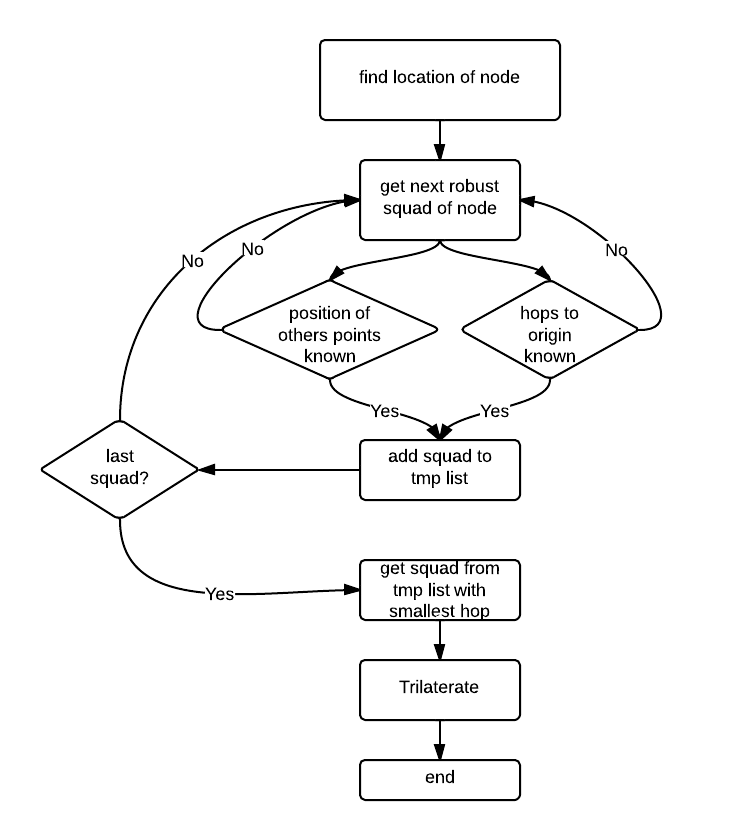
\includegraphics[width=90mm]{find_location.png}
\caption{find location of node}
\label{overflow}
\end{figure}

\subsection{Network configuration}
We tested our implementation against different types of networks configuration. The first and main one on is random graph with a minimum connectivity.
We also evaluated our solution with regular networks with particular properties.




\begin{thebibliography}{99}

\bibitem{c1} G. O. Young, ÒSynthetic structure of industrial plastics (Book style with paper title and editor),Ó 	in Plastics, 2nd ed. vol. 3, J. Peters, Ed.  New York: McGraw-Hill, 1964, pp. 15Ð64.




\end{thebibliography}




\end{document}
